% !TeX program = xelatex
% 依 2026-11-21 使用者貼上的第一章正文整合。
% 本檔包含 chapter、1.1 與 1.2；用於取代相同範圍，不要與既有章節重複載入。
% 1.3 文獻回顧沿用你在 Overleaf 已完成的內容，不由本檔取代。
% 待 1.3 結束後，再貼入「第一章_本文架構.tex」。
% 圖檔沿用 figsrc/ch01/；本檔已含圖，不要再貼「第一章_新增插圖片段.tex」。

\chapter{緒論}
\label{c:introduction}

\section{前言}
\label{sec:background}

\subsection{自主移動機械臂之發展與應用}
\label{subsec:ammr_development}

近年來，人口高齡化、勞動力結構改變與服務需求增加，使製造、物流及服務場域持續尋求具彈性的自動化方案。國際機器人聯合會（International Federation of Robotics, IFR）於2026年發布的服務型機器人產業分析指出，人力短缺是推動服務型機器人採用的重要因素，相關設備可協助執行重複性、體力負擔較高及耗時的工作，支援機構維持服務品質與營運能力。隨著環境感知與自主導航技術進步，機器人的應用也逐漸延伸至人員與設備共同活動的動態環境\cite{ifr2026impact}。

從產業規模觀察，IFR於《World Robotics 2026》發布資料中指出，在其彙整的廠商調查中，2025年專業服務型機器人銷售量接近25萬臺，較前一年增加約24\%。其中，運輸與物流類約為11.75萬臺，占約47\%，為主要應用類別；接待服務與專業清潔則分別占約22\%與18\%，如\cref{fig:ifr_service_share}所示。相關資料反映移動運輸與服務自動化的應用規模，亦顯示機器人在不同工作區域之間執行搬運與配送，已具有明確的產業需求\cite{ifr2026service}。

\begin{figure}[htbp]
    \centering
    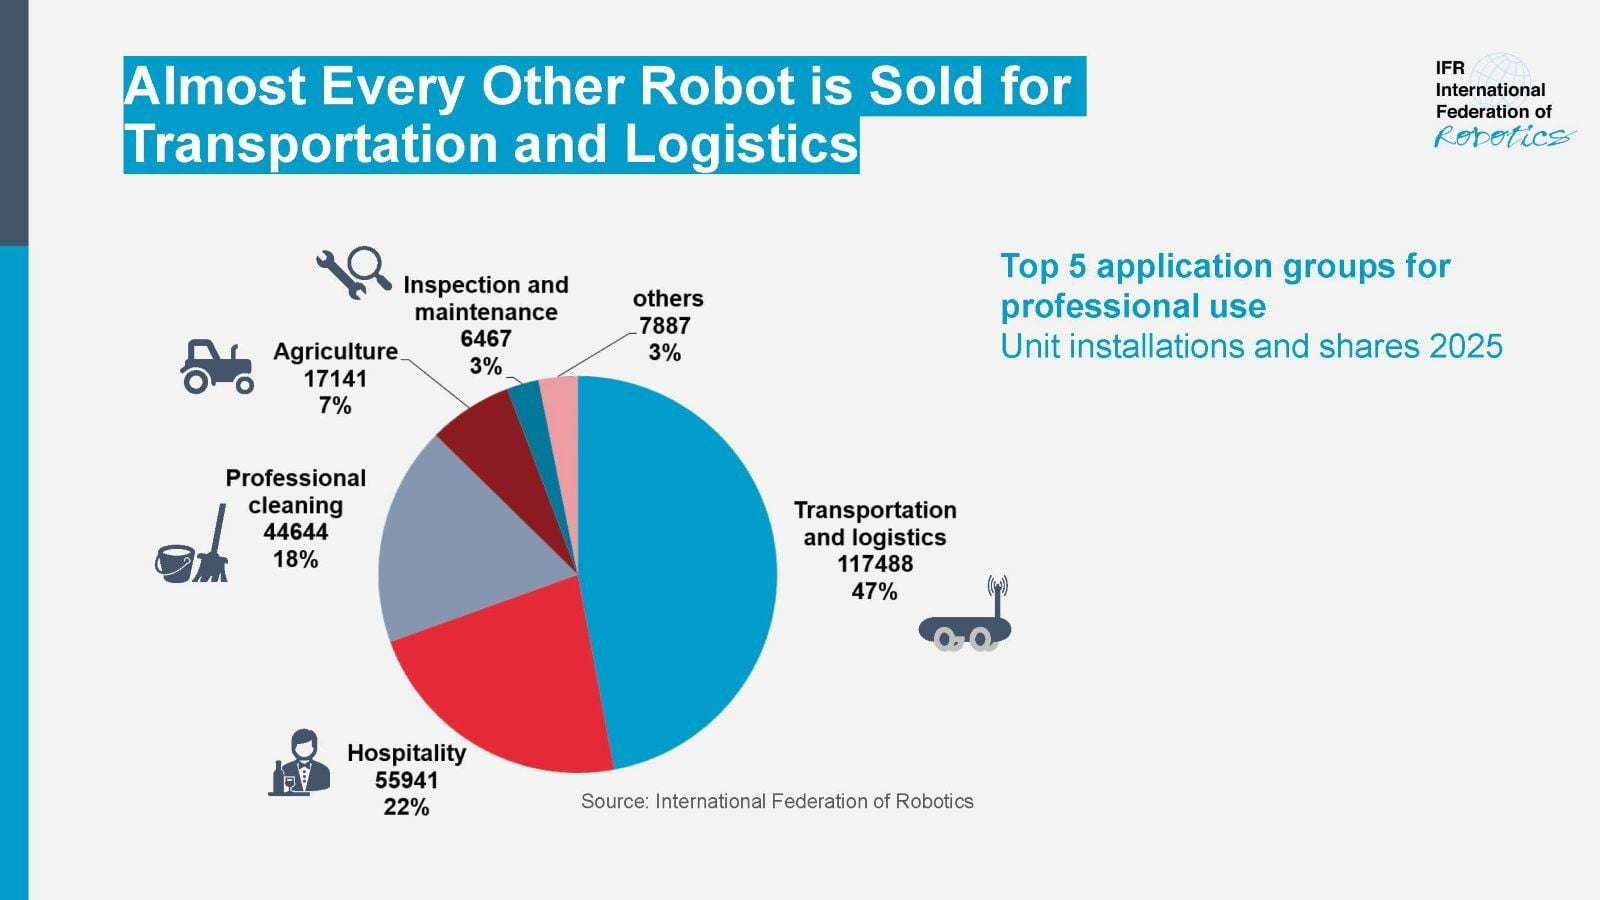
\includegraphics[width=0.95\textwidth]{figsrc/ch01/ifr_service_robots_2025_share.jpg}
    \caption{2025年專業服務型機器人主要應用類別及銷售占比\cite{ifr2026service}}
    \label{fig:ifr_service_share}
\end{figure}

在技術發展方面，IFR將人工智慧與自主性、資訊技術與實體控制的整合、人形機器人的可靠性與效率、安全與資安，以及因應人力缺口列為2026年的五項重要趨勢，如\cref{fig:ifr_robotics_trends}所示\cite{ifr2026trends}。其中，自主性、系統整合與安全等方向，與移動操作系統的發展密切相關。對於需要在共享空間中執行任務的機器人，應用需求涉及依據環境資訊調整行動、銜接不同作業階段，以及在運動過程中維持可靠的控制，使感知、規劃與執行能夠相互配合。

\begin{figure}[htbp]
    \centering
    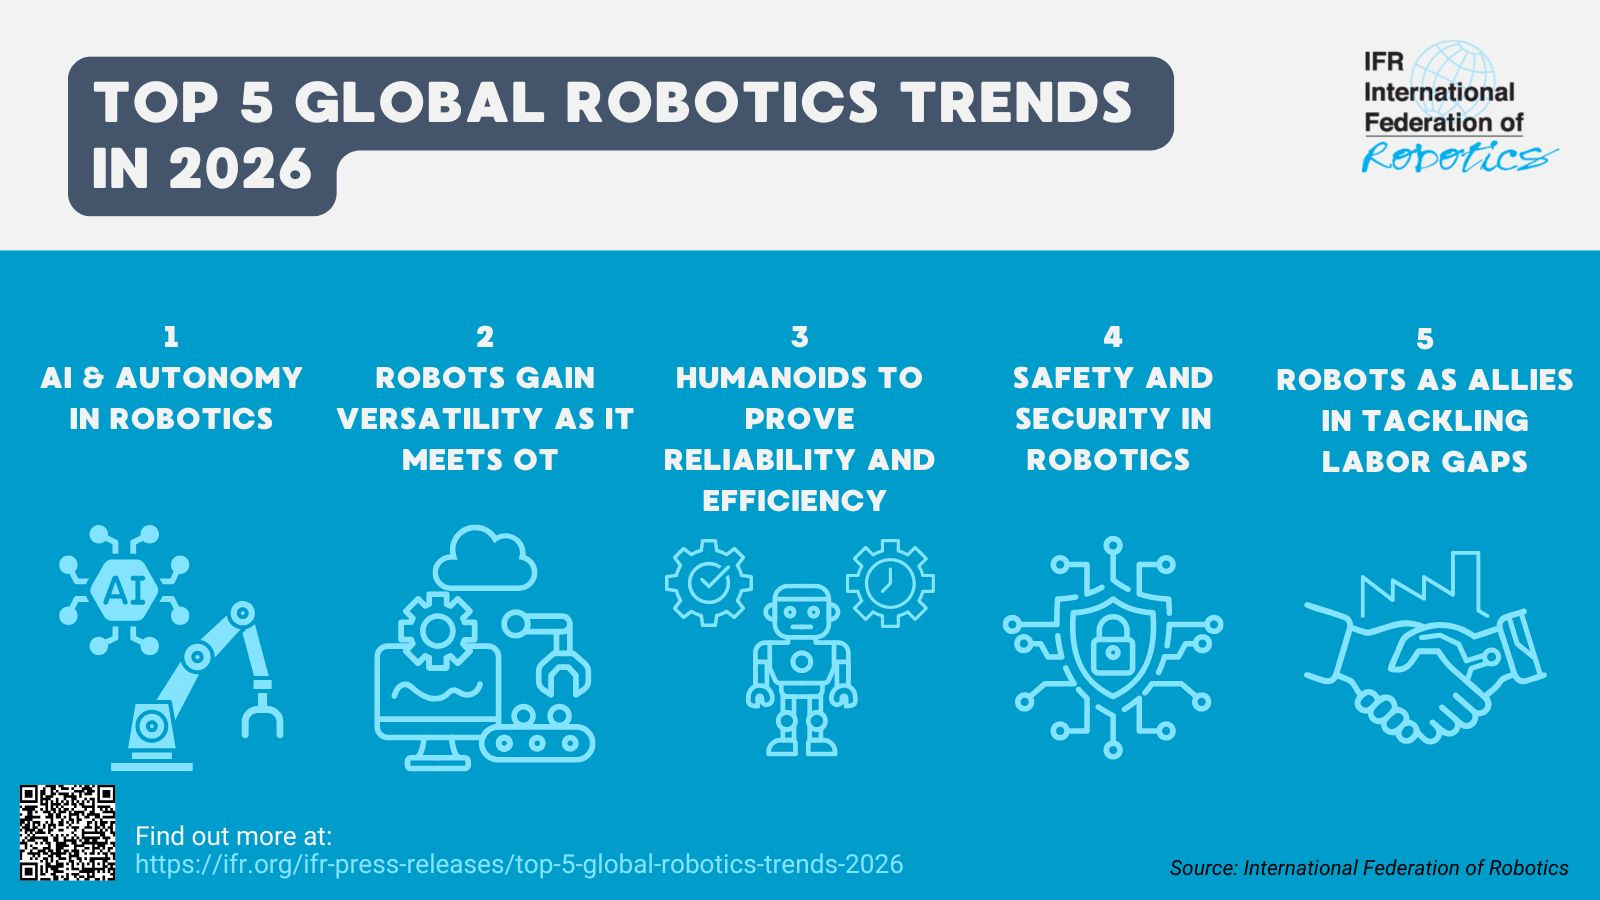
\includegraphics[width=1.0\textwidth]{figsrc/ch01/ifr_robotics_trends_2026.jpg}
    \caption{2026年全球機器人產業五項發展趨勢\cite{ifr2026trends}}
    \label{fig:ifr_robotics_trends}
\end{figure}

當任務進一步涉及物件抓取與設備操作時，機器人需要結合移動能力與手臂操作能力。自主移動機械臂（Autonomous Mobile Manipulator Robot, AMMR）整合移動底盤、機械手臂與末端執行器，藉由底盤移動延伸作業範圍，並由手臂完成物件互動，使同一系統能夠在不同位置執行操作任務。IFR於2025年的產業趨勢簡報中，亦將移動機械臂列為因應現場人力與技能短缺的彈性自動化方案之一，強調依工作位置與需求提供支援的應用價值\cite{ifr2025trends}。

移動機械臂之平台形式可依應用需求調整，如\cref{fig:mobile_manipulator_applications}所示。KUKA KMR iisy 結合移動平台與機械手臂，支援生產及物流場域的跨站作業；Hello Robot Stretch 則以室內環境中的移動與物件互動為主要設計方向\cite{kukakmriisy,hellorobotstretch4}。

\begin{figure}[htbp]
    \centering
    \begin{minipage}[b]{0.49\textwidth}
        \centering
        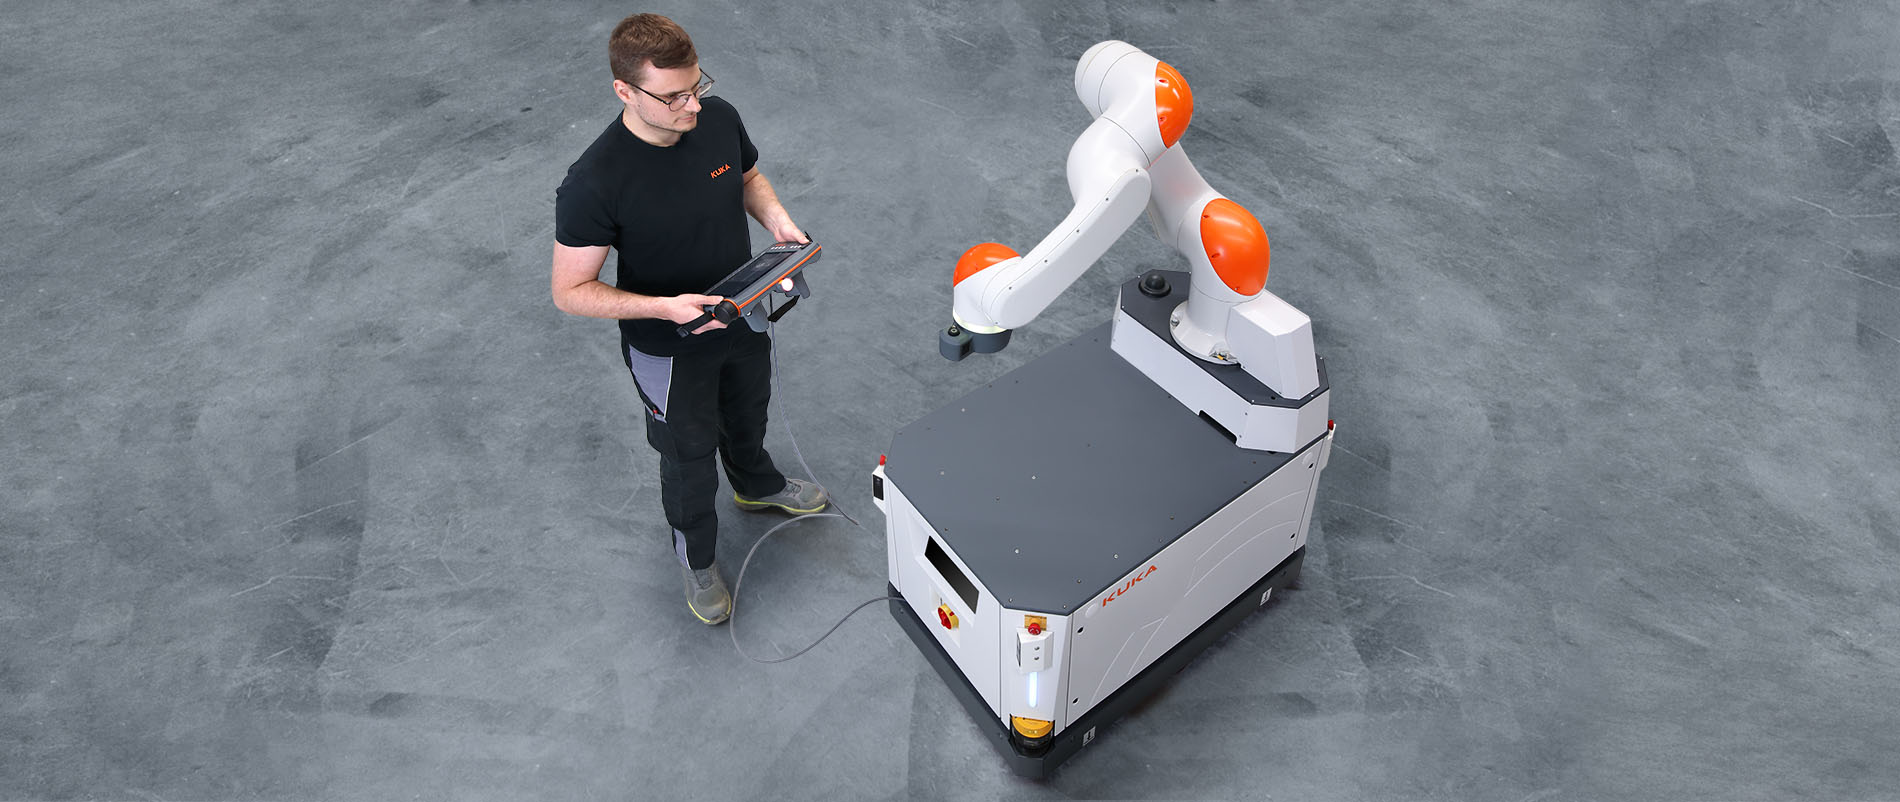
\includegraphics[width=\linewidth,height=3.2cm,keepaspectratio]{figsrc/ch01/kuka_kmr_iisy_application.jpg}
        \par\smallskip
        {\small (a) KUKA KMR iisy}
    \end{minipage}\hfill
    \begin{minipage}[b]{0.49\textwidth}
        \centering
        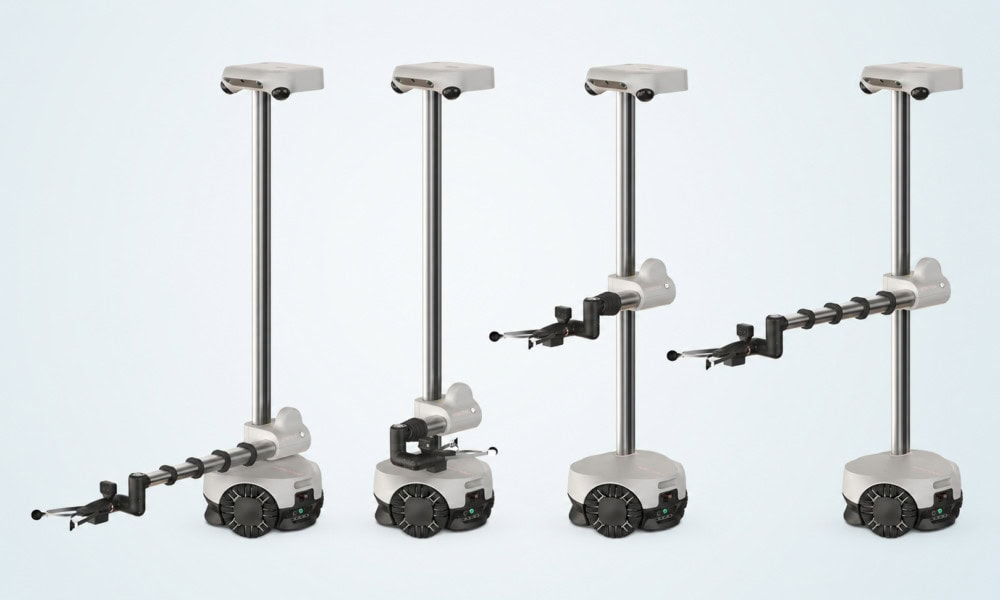
\includegraphics[width=\linewidth,height=3.2cm,keepaspectratio]{figsrc/ch01/stretch4_platform_views.jpg}
        \par\smallskip
        {\small (b) Hello Robot Stretch 4}
    \end{minipage}
    \caption{工業與室內應用導向之移動機械臂平台實例\cite{kukakmriisy,hellorobotstretch4}}
    \label{fig:mobile_manipulator_applications}
\end{figure}

\subsection{動態環境下之導航與操作需求}
\label{subsec:dynamic_navigation_manipulation}

在室內服務情境中，一項取物任務可能包含前往指定區域、辨識目標、調整操作位置、抓取與搬運等階段；若行進路徑存在關閉的門扇，或物件位於抽屜內，還需要操作環境中的可動機構。Cen Cheng 等人\cite{cencheng2026safe}將使用者需求、導航、物件辨識、抓取與遞送整合於同一架構，並以實體移動機械臂進行驗證，呈現多項功能銜接的應用需求。由此可見，移動操作的任務表現受到各階段之間的資訊傳遞與動作接續影響，評估時需要共同考量完整流程的完成情形、操作品質與時間成本。

對於門扇、櫃門與抽屜等關節式物件，操作動作還需符合鉸鏈或滑軌所允許的運動。Mittal 等人\cite{mittal2022articulated}的研究情境如\cref{fig:articulated_object_examples}所示，結合不同物件形式、場景配置與機器人平台，呈現移動與機構操作相互配合的需求。

\begin{figure}[htbp]
    \centering
    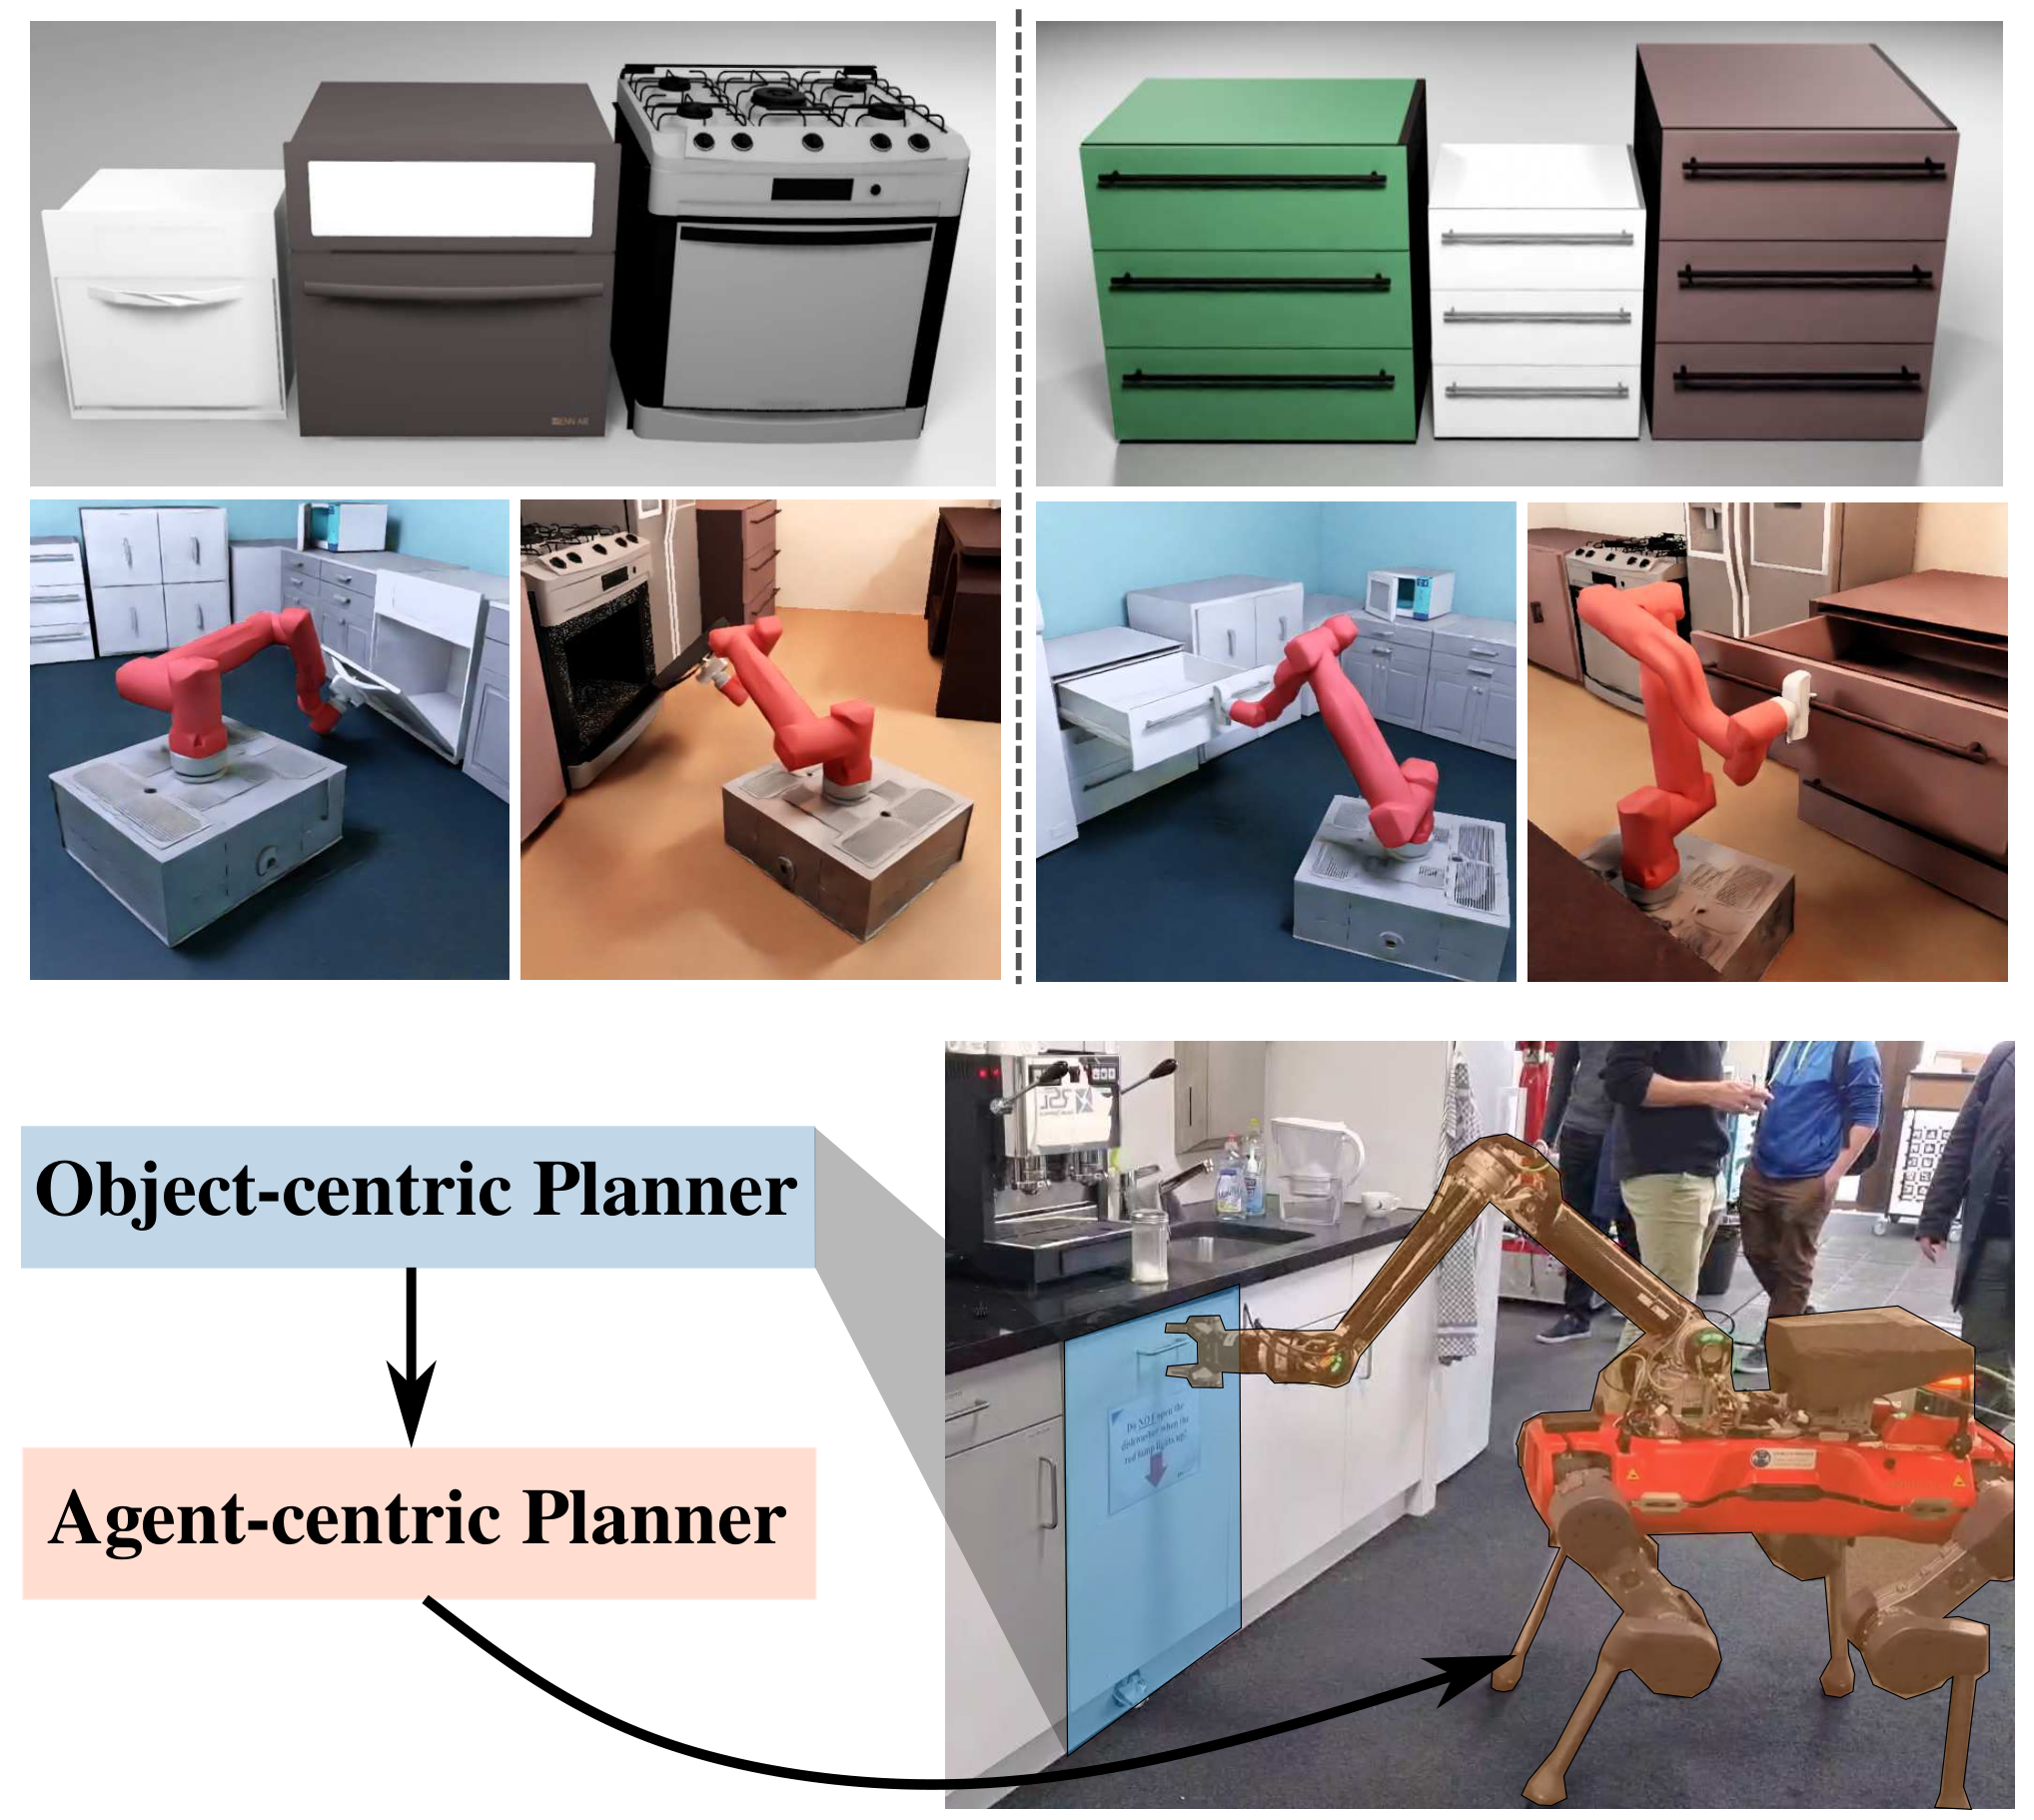
\includegraphics[width=0.80\textwidth]{figsrc/ch01/mittal2022_articulated_fig1.png}
    \caption{關節式物件操作之研究情境與系統示意，含模擬與實機場景\cite{mittal2022articulated}}
    \label{fig:articulated_object_examples}
\end{figure}

在動態環境中，底盤運動、手臂操作與目標觀測之間具有相互影響。底盤為避讓障礙而減速或轉向，會改變末端執行器與目標物的相對位置；手臂的可達範圍、關節限制與操作姿態，也會限制底盤可採取的運動。Sun 等人\cite{sun2026motion}針對移動中抓取指出，底盤與手臂的運動耦合，以及感知至執行的延遲，會影響可用的抓取時機。因此，提升任務效率需要共同安排移動進度與操作時序，並使控制器的預測能夠反映實際命令的執行特性，才能在運動限制下維持追蹤與操作品質。

基於上述產業發展與應用需求，本研究以動態室內環境中的自主移動機械臂為研究對象，探討導航、目標接近與受約束操作之間的協調問題。研究以 Tang 等人\cite{tang2024gmpc}提出之幾何模型預測控制（Geometric Model Predictive Control, GMPC）為底盤追蹤方法之基礎，結合環境感知、障礙運動預測與底盤及手臂的協同控制，並建立對應命令介面的執行動態模型。透過開門、通行與取物等任務情境，探討兼顧操作品質、動作連續性與任務效率的控制方法。

\section{研究動機與目的}
\label{sec:motivation_objectives}

\subsection{導航與操作整合之挑戰}
\label{subsec:navigation_manipulation_challenges}

自主移動機械臂執行室內任務時，需要協調底盤移動、目標接近與手臂操作。若將任務依序劃分為導航、停駐及操作等階段，雖有助於分別處理各階段的控制需求，但也可能增加等待與位置調整的時間。Burgess-Limerick 等人\cite{burgess2023motm}提出移動中操作（Manipulation on the Move, MotM）架構，使機器人在執行操作的同時，仍能朝後續任務目標移動，展示導航與操作重疊對多步驟任務效率的改善潛力。因此，如何協調底盤與手臂運動，使各任務階段有效銜接，為本研究關注的問題之一。\cref{fig:motm_research_example}為作者專案提供的連續動作模擬示意，呈現底盤行進與抓取、放置動作之間的關係\cite{burgessmotmproject}。

\begin{figure}[htbp]
    \centering
    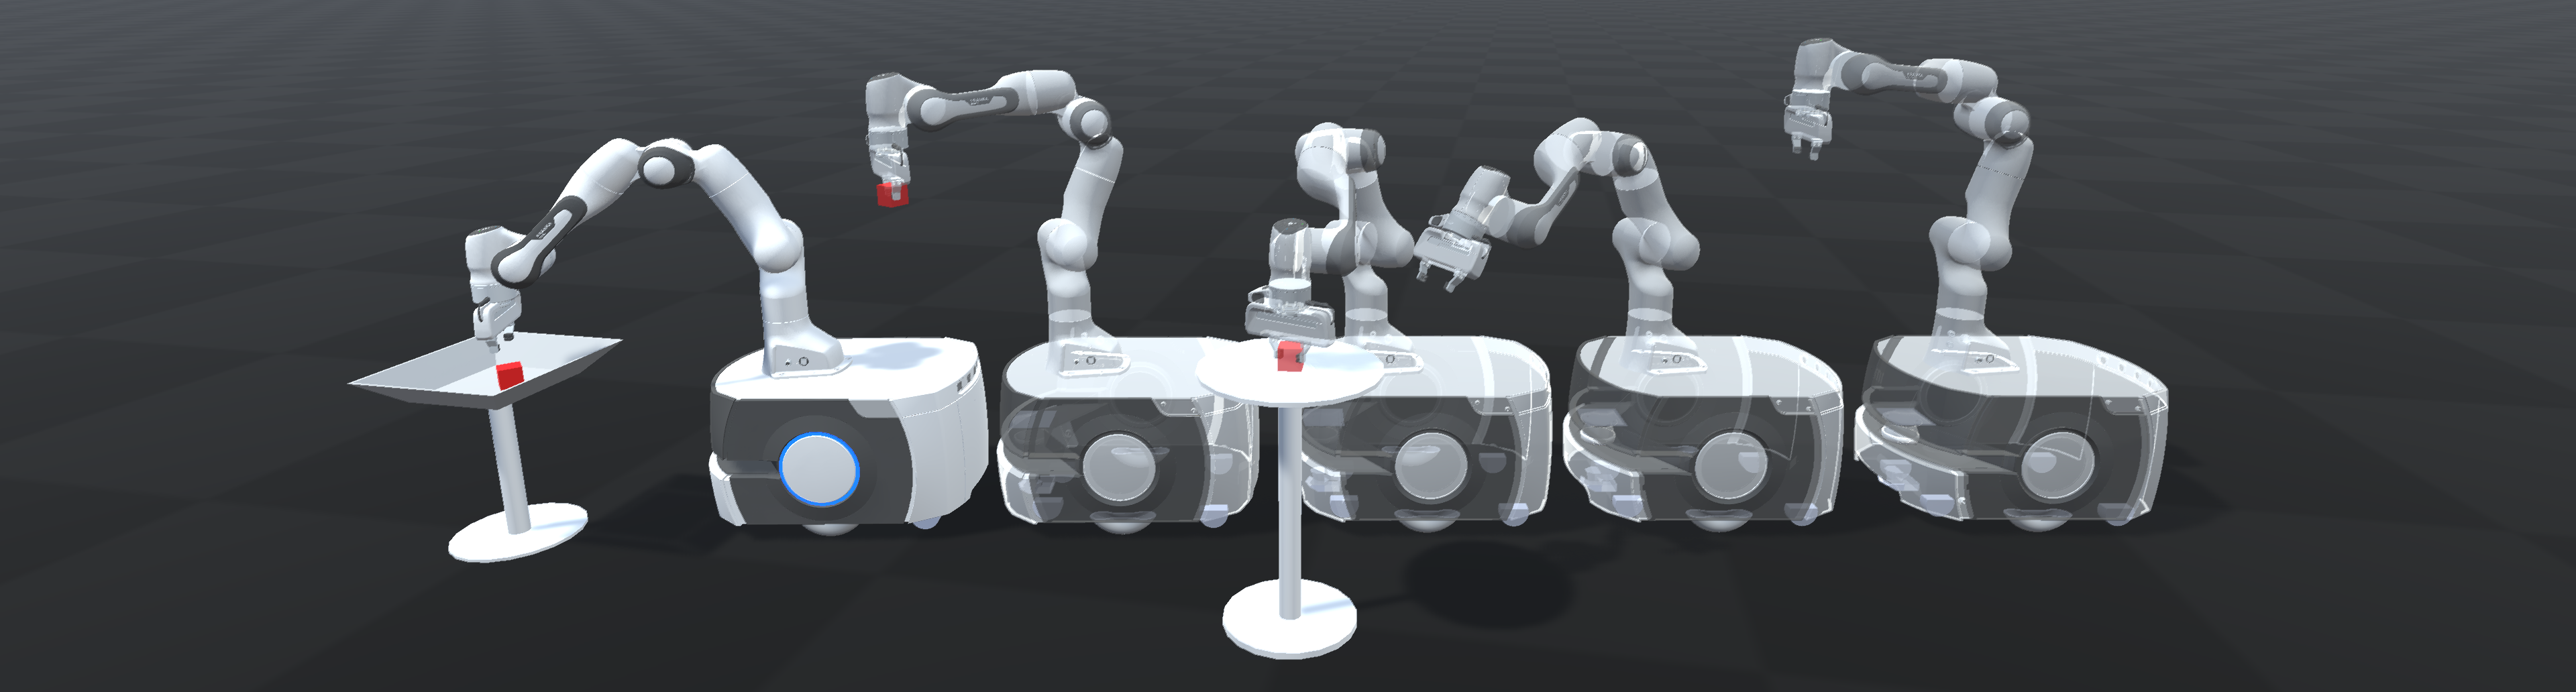
\includegraphics[width=1.0\textwidth]{figsrc/ch01/burgess2023_motm_banner.png}
    \caption{移動中抓取與放置之連續動作示意，取自作者專案之模擬圖\cite{burgess2023motm,burgessmotmproject}}
    \label{fig:motm_research_example}
\end{figure}

當底盤持續移動時，操作目標相對於機器人的位置會隨時間改變，手臂需要配合底盤運動修正末端軌跡。Sun 等人\cite{sun2026motion}針對移動抓取提出結合視覺伺服與受約束路徑規劃的方法，處理底盤與手臂的運動協調，以及有限抓取時間內的規劃需求。若環境中另有移動障礙物，底盤避障所產生的路徑調整，也需要與手臂的可達範圍及操作目標共同考量，使導航與操作之間的協調更加重要。

此外，開門等任務涉及機器人與環境機構的持續互動，除了取得操作目標的位置，還需要使末端運動符合物件的機構限制。Mittal 等人\cite{mittal2022articulated}結合 RGB-D 感知、物件操作規劃與全身最佳控制，展示移動機械臂在含有動態障礙物的環境中操作關節式物件的可行性。基於上述研究，本研究以同一全身預測控制架構為設計主線，探討如何將視覺量測、障礙資訊與機器人狀態轉換為導航及操作參考，並依任務階段更新目標與限制，使接近、抓持、開門及後續移動能夠接續執行。

\subsection{命令執行差異對預測控制之影響}
\label{subsec:command_execution_prediction}

模型預測控制（Model Predictive Control, MPC）利用系統模型預測未來運動，並依據追蹤目標與限制條件求解控制輸入，因此，預測模型與系統執行特性之間的一致性，是控制設計需要考量的因素。Grandia 等人\cite{grandia2019frequency}在足式機器人的研究中指出，未建模動態與致動器頻寬限制，可能使最佳化所得的運動無法由實際系統充分實現，並透過頻率整形的代價函數，使規劃軌跡與系統的頻寬限制相容。此研究提供了在預測控制設計中考量致動特性的依據。

對於移動機械臂，底盤與手臂可能採用不同的控制介面。Du 等人\cite{du2026wholebody}針對混合位置與速度控制的雙臂移動平台，於全身模型預測控制中處理狀態轉移及運動命令生成的一致性。本研究所使用的手臂採位置命令介面，控制輸入經積分形成關節位置設定點，再由位置控制器追蹤。因此，若直接將設定點的變化速率視為實際關節速度，便可能忽略設定點與實際關節位置之間的追蹤動態，使預測的末端運動與執行結果產生偏差。

在本研究的命令執行架構中，底盤輸入亦可能經過平滑處理、輪級運動限制及保護機制修正；若另有通訊或執行延遲，已發送而尚未生效的命令也會影響後續運動。基於此，本研究擬以關節位置與位置設定點建立增廣狀態，描述手臂命令至關節運動的追蹤關係，並將在途命令與實際放行輸入納入預測。透過與執行介面相容的模型，進一步分析命令執行動態對運動預測、末端追蹤及協同操作的影響。

\subsection{研究目的與預期貢獻}
\label{subsec:objectives_contributions}

本研究旨在建立一套適用於動態室內環境之移動機械臂預測導航與受約束操作方法。底盤追蹤方法以 Tang 等人\cite{tang2024gmpc}提出之幾何模型預測控制為基礎，進一步整合環境感知、命令執行模型與底盤及手臂的協同控制，使機器人能依環境資訊與任務需求調整運動，並銜接導航、接近、抓持與物件操作等階段。具體研究目的如下：

\begin{enumerate}
    \item \textbf{建立底盤與手臂之全身幾何預測模型。}
    結合底盤幾何運動與移動機械臂運動學，在共同預測時域內描述底盤位姿、手臂構型及末端運動，並將底盤與末端追蹤目標、關節限制及輪級運動限制納入同一最佳化問題。

    \item \textbf{建立與命令介面相容之增廣執行模型。}
    以實際關節位置與關節位置設定點描述手臂的伺服追蹤關係，並考量在途命令、實際放行輸入與執行延遲，分析執行動態建模對運動預測及末端追蹤的影響。

    \item \textbf{整合動態避障、視覺導引與受約束操作。}
    結合障礙運動預測與視覺目標資訊，建立導航、接近及操作參考，並於抓持後納入物件的機構限制。透過同一控制架構中目標與限制條件的更新，設計各任務階段之銜接方式。

    \item \textbf{建立比較與消融實驗以評估方法效能。}
    在一致的實驗條件下，分析執行模型、預測時域與協同策略對追蹤誤差、操作品質、動作連續性、任務時間及計算成本的影響，並透過開門、通行與取物情境評估方法之適用範圍。
\end{enumerate}

本研究之預期貢獻為整合幾何預測與命令執行動態之全身控制方法，以及銜接視覺導引與物件機構限制的任務參考設計，並透過比較實驗分析各項設計對追蹤品質與任務效率之作用。

% 此處接你既有的 1.3 文獻回顧及其正文。
% 1.3 結束後，再接「第一章_本文架構.tex」，由 LaTeX 自動編為 1.4。
